\documentclass[letterpaper]{article}

\setlength{\textheight}{8.875in}
\setlength{\topmargin}{0in}
\setlength{\headheight}{0in}

\usepackage{float,graphicx}
\usepackage[breaklinks=true]{hyperref}
\appto\UrlBreaks{\do\-}

\begin{document}
	\title{Classifying Higgs Boson Particles}
	
	\author{Ethan Chung\\
		{\tt\small University of Hawaii}\\
		{\tt\small ICS 635: Machine Learning}\\
		{\tt\small [redacted]@hawaii.edu}}
	
	\maketitle
	
	\section{Introduction}
	
	The Higgs Boson, observed by the Large Hadron Collider (LHC) at CERN in 2012, is an elementary particle in the Standard Model of Particle Physics believed to be responsible for giving most particles their mass through interactions. Machine learning, requiring no prior knowledge of the Higgs Boson particle, is suitable for rapid and accurate predictions. Other methods may be slower and require extensive physics expertise to accurately predict. A deeper understanding of how machine learning can be applied to this type of data could accelerate the pace of new discoveries.
	
	This project aims to develop a classifier that distinguishes events where a Higgs Boson particle is produced from events where it is not. The provided training dataset contains 50,000 labeled samples, each with 28 features. This dataset was split into 80\% for training and 20\% for validation. The features, derived from simulations of particle collisions within the ATLAS detector at the Large Hadron Collider (LHC), represent the trajectories of decay particles. The labels indicate whether an event resulted in a Higgs Boson particle. The classifier's output is a binary prediction: whether a given event produced a Higgs Boson.
	
	The training dataset, provided from the Kaggle competition, appeared to have already been pre-processed with standardization. Analysis revealed the data was centered around a mean of 0.607 and scaled to a standard deviation of 0.969. The models were trained on the training set, their hyperparameters were tuned using the validation set, and their performance was evaluated using the Area Under the Receiver Operating Characteristic (AUROC) curve on the held-out test set, also provided from the Kaggle competition and likewise contains 50,000 samples with 28 features.
	
	\section{Model Creation}
	
	Initially, a Random Forest Classifier (RFC) was employed to establish a baseline model. Despite conducting a random search using scikit-learn, varying \texttt{n\_estimators} between 50 and 500 and \texttt{max\_depth} between 0 and 10, the Area Under the Receiver Operating Characteristic (AUROC) on the validation dataset did not exceed 0.785. Subsequently, an Extreme Gradient Boosting (XGBoost) model was implemented. Notably, the AUROC on the validation dataset increased to 0.790 before any hyperparameter tuning was performed, using the following settings:
	
	\begin{table}[H]
		\centering
		\caption{Initial XGBoost Hyperparameters}
		\begin{tabular}{ll}
			\hline
			Hyperparameter & Value \\
			\hline
			\texttt{learning\_rate} & 0.1 \\
			\texttt{n\_estimators} & 1000 \\
			\texttt{max\_depth} & 10 \\
			\texttt{min\_child\_weight} & 1 \\
			\texttt{gamma} & 0 \\
			\texttt{subsample} & 0.8 \\
			\texttt{colsample\_bytree} & 0.8 \\
			\texttt{objective} & \texttt{binary:logistic} \\
			\texttt{n\_jobs} & -1 \\
			\texttt{random\_state} & 42 \\
			\texttt{scale\_pos\_weight} & 1 \\
			\hline
		\end{tabular}
		\label{tab:initial_xgboost_params}
	\end{table}
	
	These settings were copied from a sample XGBoost tutorial and therefore do not reflect any specific hyperparameter optimization. A possible reason for XGBoost performing better is due to the dataset being pre-processed through standardization, which helps with model convergence and benefits from features being scaled similarly.
	
	An AdaBoostClassifier was also evaluated, using the ExtraTreesClassifier method with the following hyperparameters:
	
	\begin{table}[H]
		\centering
		\caption{AdaBoost with ExtraTreesClassifier Hyperparameters}
		\begin{tabular}{ll}
			\hline
			Hyperparameter & Value \\
			\hline
			\texttt{ExtraTreesClassifier(n\_estimators)} & 400 \\
			\texttt{ExtraTreesClassifier(max\_features)} & 30 \\
			\texttt{ExtraTreesClassifier(max\_depth)} & 12 \\
			\texttt{ExtraTreesClassifier(min\_samples\_leaf)} & 100 \\
			\texttt{ExtraTreesClassifier(min\_samples\_split)} & 100 \\
			\texttt{ExtraTreesClassifier(n\_jobs)} & -1 \\
			\texttt{AdaBoostClassifier(n\_estimators)} & 20 \\
			\texttt{AdaBoostClassifier(algorithm)} & \texttt{SAMME.R} \\
			\texttt{AdaBoostClassifier(learning\_rate)} & 0.75 \\
			\texttt{AdaBoostClassifier(random\_state)} & 42 \\
			\hline
		\end{tabular}
		\label{tab:adaboost_params}
	\end{table}
	
	This yielded an AUROC of 0.803064797627409 on the validation set without any hyperparameter tuning. However, the XGBoost model was chosen for further optimization for no particular reason.
	
	\section{Hyperparameter Tuning}
	
	Hyperparameter optimization was performed using the \texttt{XGBoostClassifier} from scikit-learn, in conjunction with Hyperopt and the Tree-based Parzen Estimators (TPE) algorithm. The objective was to maximize the AUROC score on the validation dataset over a maximum of 100 trials.
	
	The hyperparameter search space was defined as follows:
	
	\begin{table}[H]
		\centering
		\caption{Hyperparameter Search Space}
		\begin{tabular}{ll}
			\hline
			Hyperparameter & Search Space \\
			\hline
			\texttt{n\_estimators} & \texttt{choice([300, 500, 1000])} \\
			\texttt{max\_depth} & \texttt{choice([10, 12, 15])} \\
			\texttt{learning\_rate} & \texttt{loguniform(np.log(0.01), np.log(1))} \\
			\texttt{min\_child\_weight} & \texttt{uniform(1, 5)} \\
			\texttt{gamma} & \texttt{uniform(0, 5)} \\
			\texttt{reg\_lambda} & \texttt{uniform(0.0, 1.0)} \\
			\texttt{colsample\_bytree} & \texttt{uniform(0.5, 1.0)} \\
			\hline
		\end{tabular}
		\label{tab:hyperparameter_search_space}
	\end{table}
	
	The optimal hyperparameters, yielding an AUROC of 0.802 on the validation set, were found to be:
	
	\begin{table}[H]
		\centering
		\caption{Final Optimal Hyperparameters}
		\begin{tabular}{ll}
			\hline
			Hyperparameter & Value \\
			\hline
			\texttt{colsample\_bytree} & 0.634773166725724 \\
			\texttt{gamma} & 1.5641000812832375 \\
			\texttt{learning\_rate} & 0.010417885267605457 \\
			\texttt{max\_depth} & 12 \\
			\texttt{min\_child\_weight} & 1.4294921423171645 \\
			\texttt{n\_estimators} & 1000 \\
			\texttt{reg\_lambda} & 0.8143493244635522 \\
			\hline
		\end{tabular}
		\label{tab:optimal_hyperparameters}
	\end{table}
	
	The AUROC curve for the final XGBoost model is:
	
	\begin{figure}[H]
		\centering
		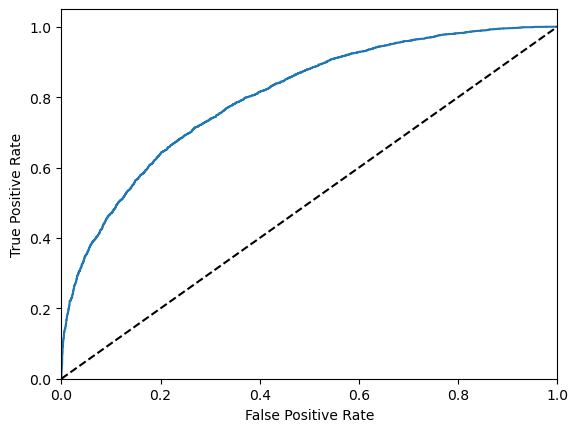
\includegraphics[width=0.7\linewidth]{XGBoostAUROC}
		\caption{AUROC curve of final XGBoost model}
		\label{fig:xgboostauroc}
	\end{figure}
	
	\section{Experimentation with AutoML Techniques}
	
	Automated Machine Learning (AutoML) techniques aim to streamline the model development process by automating tasks such as feature engineering, model selection, and hyperparameter tuning. Among various AutoML frameworks, AutoGluon in particular stands out for its strong performance on tabular data. In this experiment, AutoGluon was employed to explore its potential for classifying Higgs Boson production events. Specifically, the \texttt{TabularPredictor} from the \texttt{autogluon.tabular} module was utilized. The training was conducted using the provided train dataset, with the 'label' column designated as the target variable. The predictor was configured for binary classification with the AUROC as the evaluation metric. The fitted model was then used to generate predictions on the provided test dataset, and the resulting probabilities were saved in a submission file.
	
	The model training was conducted using the University of Hawaii at Manoa's HPC cluster (Koa). GPU-accelerated training was attempted, but due to the difficulty of requesting multiple GPUs, AutoGluon was performed using only CPU. The nodes requested used 48 cores and 128GB to 256GB of RAM depending on node availability, which completed each batch of training in around 6 to 8 hours. A total of 9 models were created using AutoGluon: three models used the \texttt{best\_quality} preset, and the rest used the \texttt{experimental\_quality} preset. Hyper-parameter tuning was performed on some of these trials, using a random searcher, a local scheduler, and 5 trials per model and using the default hyper-parameter tuning preset, as defined in the AutoGluon GitHub repository: \href{https://github.com/autogluon/autogluon/blob/e9fb676160be13467d321df24fddc60f152c2813/tabular/src/autogluon/tabular/configs/hyperparameter_configs.py#L8-L38}{\textit{AutoGluon Hyperparameter Config}}. The quality presets are also defined in their documentation: \href{https://auto.gluon.ai/stable/api/autogluon.tabular.TabularPredictor.fit.html}{\textit{TabularPredictor.fit}}.
	
	Across all nine models, AutoGluon identified the \texttt{WeightedEnsemble\_L3} model as the top performer consistently. A \texttt{WeightedEnsemble} is an ensemble learning technique that combines the predictions from multiple individual models, known as base learners, to produce more accurate and robust predictions than any single model alone. It works by assigning different weights to each model's predictions, giving more importance to models that perform better. This approach leverages the strengths of individual models and mitigates their weaknesses. Bagging, or Bootstrap Aggregating, is a specific ensemble method where multiple models are trained independently on random subsets of the training data, sampled with replacement. The predictions from these models are then aggregated by averaging to make a final prediction. Moreover, bagging also reduces variance and mostly mitigates overfitting problems. AutoGluon reports this process in more detail in their documentation: \href{https://auto.gluon.ai/dev/tutorials/tabular/how-it-works.html}{\textit{How it works}}.
	
	Due to the complexity of manually analyzing the internal workings of each AutoML-trained model, the focus will be on detailing the best-performing ensemble (achieved in Trial 3). The logs for each trained model is available in the GitHub repository.
	
	\begin{itemize}
		\item The best-performing ensemble model, \texttt{WeightedEnsemble\_L3}, achieved an AUROC of 0.819845 on the validation dataset. On this particular model, 44444 rows were used for the training set, and the other 5556 rows were used as the validation set.
		\item AutoGluon trained a total of 428 models of the following types:
		\begin{itemize}
			\item \texttt{StackerEnsembleModel\_XT}
			\item \texttt{StackerEnsembleModel\_LGB}
			\item \texttt{StackerEnsembleModel\_CatBoost}
			\item \texttt{WeightedEnsembleModel}
			\item \texttt{StackerEnsembleModel\_XGBoost}
			\item \texttt{StackerEnsembleModel\_TabularNeuralNetTorch}
			\item \texttt{StackerEnsembleModel\_NNFastAiTabular}
			\item \texttt{StackerEnsembleModel\_KNN}
			\item \texttt{StackerEnsembleModel\_RF}
		\end{itemize}
		\item The ensemble used 8-fold cross-validation bagging and a three-level multi-layer stack-ensemble.
		\item AutoGluon utilized all 28 input features without performing any additional feature engineering.
		\item AutoGluon performs early stopping if there are no improvements between epochs or when an individual model exceeds the time limit allocated for training that particular model.
	\end{itemize}
	
	The ensemble weights for the \texttt{WeightedEnsemble\_L3} model were as follows:
	
	\begin{table}[H]
		\centering
		\caption{WeightedEnsemble\_L3 Model Weights and Validation AUROC}
		\begin{tabular}{lcc}
			\hline
			Model & Weight & Validation AUROC \\
			\hline
			\texttt{NeuralNetFastAI\_r88\_BAG\_L2} & 0.24 & 0.8192 \\
			\texttt{LightGBM\_BAG\_L2/T3} & 0.12 & 0.8176 \\
			\texttt{NeuralNetFastAI\_BAG\_L2/be8d3\_00003} & 0.12 & 0.8182 \\
			\texttt{NeuralNetTorch\_r135\_BAG\_L2/db12d\_00000} & 0.12 & 0.8178 \\
			\texttt{NeuralNetFastAI\_r172\_BAG\_L2} & 0.08 & 0.8181 \\
			\texttt{NeuralNetTorch\_r36\_BAG\_L2/5ead3\_00002} & 0.08 & 0.8184 \\
			\texttt{CatBoost\_BAG\_L2/T3} & 0.04 & 0.8184 \\
			\texttt{RandomForest\_r195\_BAG\_L2} & 0.04 & 0.8110 \\
			\texttt{ExtraTrees\_r178\_BAG\_L2} & 0.04 & 0.8159 \\
			\texttt{RandomForest\_r166\_BAG\_L2} & 0.04 & 0.8134 \\
			\texttt{NeuralNetFastAI\_r4\_BAG\_L2} & 0.04 & 0.8186 \\
			\texttt{NeuralNetTorch\_r36\_BAG\_L2/5ead3\_00004} & 0.04 & 0.8179 \\
			\hline
		\end{tabular}
		\label{tab:ensemble_weights_2}
	\end{table}
	
	Interestingly, AutoGluon did not select XGBoost for the final ensemble, choosing NeuralNetFastAI instead. FastAI, a library built on PyTorch, simplifies deep learning by offering high-level tools that enable quick development of state-of-the-art models. The specific model chosen, \texttt{NeuralNetFastAI\_r88\_BAG\_L2}, indicates that it was the 88th iteration of the NeuralNetFastAI model, trained with bagging, and was incorporated into the second layer (Level 2) of a stacked ensemble. This implies that the model was trained using the predictions generated by the base models in the first layer (Level 1) as input features.
	
	A key observation is that AutoGluon's weighted ensemble did not solely select the top 12 models by validation AUROC. Instead, it incorporated models with scores ranging from 0.8110 to 0.8192. This is likely to diversify the ensemble by leveraging strengths and weaknesses of individual models to enhance robustness of the ensemble, and could be another method of reducing overfitting.
	
	\section{Conclusion}
		
	Following evaluation on the held-out test set, submission files for the manually tuned XGBoost model and AutoGluon's \texttt{WeightedEnsemble\_L3} model were uploaded to Kaggle. The public leaderboard, which represents 30\% of the test data, yielded AUROC scores of 0.80438 for the XGBoost model (a 0.0028 increase compared to validation) and 0.82167 for the weighted ensemble model (a 0.001866 increase compared to validation). These scores demonstrate that both models successfully generalized to unseen data and did not overfit the validation set. Additionally, given the inherent stability of fundamental physics laws, it is reasonable to expect that the models' performance on simulated data will remain reliable over time.
	
	This also highlights the potential of AutoML tools like AutoGluon, though they present a unique challenge in Explainable AI (XAI). The abstracted nature of AutoML processes makes it more difficult to understand the model's decision-making processes without digging into the source code. This is a common argument against using AutoML tools. A suggested practice, however, is to leverage AutoGluon for quick experimentation with various models and parameters with very little effort, using the resulting insights as a starting point for developing further models.
	
	\section{Code Availability}
	All code and results related to this report is hosted at \url{https://github.com/echung32/ics635-higgs-boson/}, alongside the best final model for AutoGluon.
	
	\section{Kaggle Submission}
	
	\begin{itemize}
	    \item \textbf{Username:} echung32
		\item \textbf{Public Leaderboard Rank:} \#2 (effectively \#1, due to the leading submission's suspected use of the actual test set).
		\item \textbf{Private Leaderboard Rank:} TBD
	\end{itemize}

\end{document}